\begin{subsection}{The \texttt{draw} command}
The most common command in \MP{} is the \texttt{draw} command.  This command is used to draw paths or pictures.  In order to draw a path from \texttt{z1:=(0,0)} to \texttt{z2:=(54,18)} to \texttt{z3:=(72,72)}, we should first decide how we want the path to look.  For example, if we want these points to simply be connected by line segments, then we use \begin{center}\verb|draw z1--z2--z3;|\end{center}  However, if we want a smooth path between these points, we use \begin{center}\verb|draw z1..z2..z3;|\end{center}  In order to specify the direction of the path at the points, we use the \texttt{dir} operator.  In Figure \ref{fig:draw1} we see that the smooth path is horizontal at \texttt{z1}, a 45\textdegree\ angle at \texttt{z2}, and vertical at \texttt{z3}.  These constraints on the B\'{e}zier curve are imposed by \begin{center}\verb|draw z1{right}..z2{dir 45}..{up}z3;|\end{center}
\begin{figure}[ht]
	\begin{center}\textattachfile[color={0 0 0},mimetype={text/plain}]{draw_1.mp}{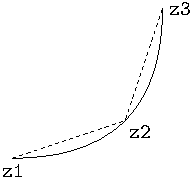
\includegraphics{draw_1}}\end{center}
	\caption{\texttt{draw} examples}\label{fig:draw1}
\end{figure}
Notice that \verb|z2{dir 45}| forces the \textit{outgoing} direction at \texttt{z2} to be 45\textdegree.  This implies an \textit{incoming} direction at \texttt{z2} of 45\textdegree.  In order to require different incoming and outgoing directions, we would use \begin{center}\verb|draw z1{right}..{dir |$\theta_i$\verb|}z2{dir |$\theta_o$\verb|}..{up}z3;|\end{center} where $\theta_i$ and $\theta_o$ are the incoming and outgoing directions, respectively.
\end{subsection}
